%%%%%%%%%%%%%%%%%%%%%%%%%%%%%%%%%%%%%%%%%%%%%%%%%%%%%%%%%%%%%%%%%%%%%%%%%%%%%%%%
%
% Template license:
% CC BY-NC-SA 3.0 (http://creativecommons.org/licenses/by-nc-sa/3.0/)
%
%%%%%%%%%%%%%%%%%%%%%%%%%%%%%%%%%%%%%%%%%%%%%%%%%%%%%%%%%%%%%%%%%%%%%%%%%%%%%%%%

%----------------------------------------------------------------------------------------
%	PACKAGES AND OTHER DOCUMENT CONFIGURATIONS
%----------------------------------------------------------------------------------------

\documentclass[
11pt, % The default document font size, options: 10pt, 11pt, 12pt
%oneside, % Two side (alternating margins) for binding by default, uncomment to switch to one side
%chapterinoneline,% Have the chapter title next to the number in one single line
spanish,
singlespacing, % Single line spacing, alternatives: onehalfspacing or doublespacing
%draft, % Uncomment to enable draft mode (no pictures, no links, overfull hboxes indicated)
%nolistspacing, % If the document is onehalfspacing or doublespacing, uncomment this to set spacing in lists to single
%liststotoc, % Uncomment to add the list of figures/tables/etc to the table of contents
%toctotoc, % Uncomment to add the main table of contents to the table of contents
parskip, % Uncomment to add space between paragraphs
%codirector, % Uncomment to add a codirector to the title page
headsepline, % Uncomment to get a line under the header
]{MastersDoctoralThesis} % The class file specifying the document structure



%----------------------------------------------------------------------------------------
%	INFORMACIÓN DE LA MEMORIA
%----------------------------------------------------------------------------------------

\thesistitle{Sistema de monitoreo remoto de centrales de alarma de incendio de la marca Simplex} % El títulos de la memoria, se usa en la carátula y se puede usar el cualquier lugar del documento con el comando \ttitle

% Nombre del posgrado, se usa en la carátula y se puede usar el cualquier lugar del documento con el comando \degreename
%\posgrado{Carrera de Especialización en Sistemas Embebidos} 
%\posgrado{Carrera de Especialización en Internet de las Cosas} 
%\posgrado{Carrera de Especialización en Intelegencia Artificial}
\posgrado{Maestría en Sistemas Embebidos} 
%\posgrado{Maestría en Internet de las cosas}

\author{Esp. Ing. Daniel Marquez} % Tu nombre, se usa en la carátula y se puede usar el cualquier lugar del documento con el comando \authorname

\director{Dra. Alejandra Aguirre (IBCN UBA-CONICET)} % El nombre del director, se usa en la carátula y se puede usar el cualquier lugar del documento con el comando \dirname
\codirector{Nombre del codirector (pertenencia)} % El nombre del codirector si lo hubiera, se usa en la carátula y se puede usar el cualquier lugar del documento con el comando \codirname.  Para activar este campo se debe descomentar la opción "codirector" en el comando \documentclass, línea 23.

\juradoUNO{Mg. Ing. Edgardo Torrelli (FIUBA)} % Nombre y pertenencia del un jurado se usa en la carátula y se puede usar el cualquier lugar del documento con el comando \jur1name
\juradoDOS{Mg. Ing. Sergio Burgos (UTN-FRP)} % Nombre y pertenencia del un jurado se usa en la carátula y se puede usar el cualquier lugar del documento con el comando \jur2name
\juradoTRES{Mg. Ing. Mariano Mondani (FIUBA)} % Nombre y pertenencia del un jurado se usa en la carátula y se puede usar el cualquier lugar del documento con el comando \jur3name

\ciudad{Ciudad Autónoma de Buenos Aires}
%\ciudad{ciudad de Mendoza}

\fechaINICIO{junio de 2021}
\fechaFINAL{diciembre de 2022}


\keywords{Sistemas embebidos, FIUBA} % Keywords for your thesis, print it elsewhere with \keywordnames


\begin{document}


\frontmatter % Use roman page numbering style (i, ii, iii, iv...) for the pre-content pages

\pagestyle{plain} % Default to the plain heading style until the thesis style is called for the body content


%----------------------------------------------------------------------------------------
%	RESUMEN - ABSTRACT 
%----------------------------------------------------------------------------------------

\begin{abstract}
\addchaptertocentry{\abstractname} % Add the abstract to the table of contents
%
%The Thesis Abstract is written here (and usually kept to just this page). The page is kept centered vertically so can expand into the blank space above the title too\ldots
\centering

Esta memoria describe el desarrollo de un sistema embebido distribuido para el monitoreo de sistemas de detección de incendio. El trabajo corresponde a la continuación de desarrollos tecnológicos por parte de la empresa Isolse srl. La finalidad de la organización es ofrecer a sus clientes un sistema de monitoreo de centrales de alarma de incendio, con la capacidad de notificar a los usuarios de forma remota ante la presencia de un evento de alarma o falla en sus instalaciones.

El equipo se diseña mediante los conocimientos de certificación de sistemas electrónicos, estudio de sistemas críticos y sistemas embebidos distribuidos. De esta manera se provee una plataforma funcional con el potencial de convertirse en un producto comercial certificable.
			

\end{abstract}

%----------------------------------------------------------------------------------------
%	CONTENIDO DE LA MEMORIA  - AGRADECIMIENTOS
%----------------------------------------------------------------------------------------

\begin{acknowledgements}
%\addchaptertocentry{\acknowledgementname} % Descomentando esta línea se puede agregar los agradecimientos al índice
\vspace{1.5cm}

Esta sección es para agradecimientos personales y es totalmente \textbf{OPCIONAL}.  

\end{acknowledgements}

%----------------------------------------------------------------------------------------
%	LISTA DE CONTENIDOS/FIGURAS/TABLAS
%----------------------------------------------------------------------------------------

\tableofcontents % Prints the main table of contents

\listoffigures % Prints the list of figures

\listoftables % Prints the list of tables


%----------------------------------------------------------------------------------------
%	CONTENIDO DE LA MEMORIA  - DEDICATORIA
%----------------------------------------------------------------------------------------

\dedicatory{\textbf{Dedicado a... [OPCIONAL]}}  % escribir acá si se desea una dedicatoria

%----------------------------------------------------------------------------------------
%	CONTENIDO DE LA MEMORIA  - CAPÍTULOS
%----------------------------------------------------------------------------------------

\mainmatter % Begin numeric (1,2,3...) page numbering

\pagestyle{thesis} % Return the page headers back to the "thesis" style

% Incluir los capítulos como archivos separados desde la carpeta Chapters

% Chapter 1

\chapter{Introducción general} % Main chapter title

\label{Chapter1} % For referencing the chapter elsewhere, use \ref{Chapter1}
\label{IntroGeneral}

%----------------------------------------------------------------------------------------

% Define some commands to keep the formatting separated from the content
\newcommand{\keyword}[1]{\textbf{#1}}
\newcommand{\tabhead}[1]{\textbf{#1}}
\newcommand{\code}[1]{\texttt{#1}}
\newcommand{\file}[1]{\texttt{\bfseries#1}}
\newcommand{\option}[1]{\texttt{\itshape#1}}
\newcommand{\grados}{$^{\circ}$}

%----------------------------------------------------------------------------------------

%\section{Introducción}
%citas \citep{ARTICLE:1}
%----------------------------------------------------------------------------------------
%s
En el presente capítulo se describe el funcionamiento de un sistema de detección de incendio convencional, la lógica que suelen tener los protocolos de notificación de eventos, y las tecnologías actuales de monitoreo remoto que existen. Finalmente se detallan los motivos del proyecto enfocado a las necesidades del mercado argentino. 


\section{Sistemas de alarma de incendio.}
%
La detección de incendios es una herramienta preventiva clave para la seguridad humana \citep{rev_innov_1}, a su vez corresponde a un elemento de vital importancia para la evacuación exitosa ante situaciones de emergencia. En diferentes ciudades del mundo son considerados requisitos indispensables para poder categorizar a un establecimiento como habitable.

A partir del código de edificación dispuesto desde el año 2019 en la Ciudad de Buenos Aires \citep{cod_edif}, se establece que los sistemas de detección de alarma de incendio (SDAI) son requisitos obligatorios para diferentes tipos de recintos. A su vez, se debe considerar que contar con un SDAI no significa que el recinto se encuentre debidamente protegido, esto se evidencia en la Ley 5920 \citep{ley_5920}. En la que se exige a los establecimientos presentar un sistema de autoprotección \citep{rev_innov_2}, en el cual se incluye entre sus elementos obligatorios un plan de evacuación y la designación de personas con un rol específico, en el caso de requerir ejecutar procedimientos de emergencia. En otras palabras, a pesar de que efectivamente un SDAI es un elemento invaluable para una edificación, desde un punto de vista legal por sí mismo no es suficiente como única medida de protección. 

Los protocolos de evacuación usualmente se apoyan en sistemas automatizados y especifican la serie de acciones, modos, pautas y tiempos estimados de evacuación. Los beneficios más significativos de contar con un SDAI se pueden reducir en tres principales: evitar la inhalación de humo, detección temprana y monitoreo ininterrumpido. El beneficio primordial es la detección temprana, ya que minimiza el tiempo de reacción de los ocupantes y en conjunto con un sistema de notificación eficiente, pueden dar inicio a la toma de acciones por parte del personal especializado, lo que disminuye el tiempo total de evacuación. \citep{utn_1}\citep{plan_evac}.
\subsection{Sistemas de detección de alarma de incendio convencionales}
%

En la figura \ref{fig:sdai_conv} podemos observar la distribución de un SDAI básico, es evidente que los sistemas de detección de incendio cuentan con dos componentes clave, con un objetivo específico:
\begin{itemize}
\item Circuito de detección: circuito eléctrico que comprende aquellos dispositivos cuya finalidad es detectar (mediante el monitoreo de fenómenos físicos) los focos de incendio. Por ejemplo: detectores de humo, iónicos, llama, avisadores manuales, etc.
\item Circuito de notificación: a diferencia del circuito de detección, estos dispositivos reaccionan una vez detectado el foco de incendio. La función de estos dispositivos es dar aviso a los ocupantes del recinto en caso de una alarma de incendio. Por ejemplo: sirenas, luces estroboscópicas, sistemas de audio, accionamiento de contactos eléctricos, etc.
\end{itemize}
\begin{figure}[ht]
    \centering
    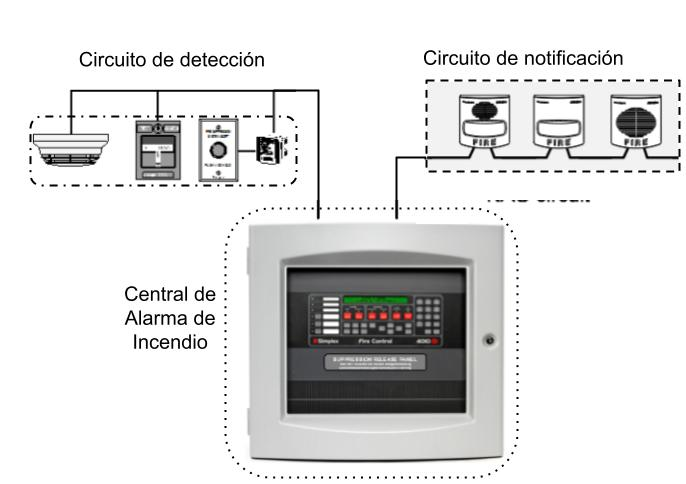
\includegraphics[scale=.45]{./Figures/sdai_conv.jpg}
    \caption{Esquema de un SDAI básico.}
    \label{fig:sdai_conv}
\end{figure}

Por lo general una central de alarma de incendio (CAI) realiza las tareas de monitorear, registrar, notificar y finalmente reaccionar a eventos de falla y/o alarma en la instalación. Todos los eventos cuentan con notificación visual y sonora en la CAI, sin embargo el accionamiento del circuito de notificación depende del protocolo de evacuación implementado. La figura \ref{fig:flujo_conv} aclara el flujo de procesamiento usual de un evento de alarma, primero la etapa de detección, luego reporte en en la CAI con los datos del dispositivo y finalmente una etapa de notificación a los usuario según el protocolo de evacuación.

\begin{figure}[ht]
    \centering
    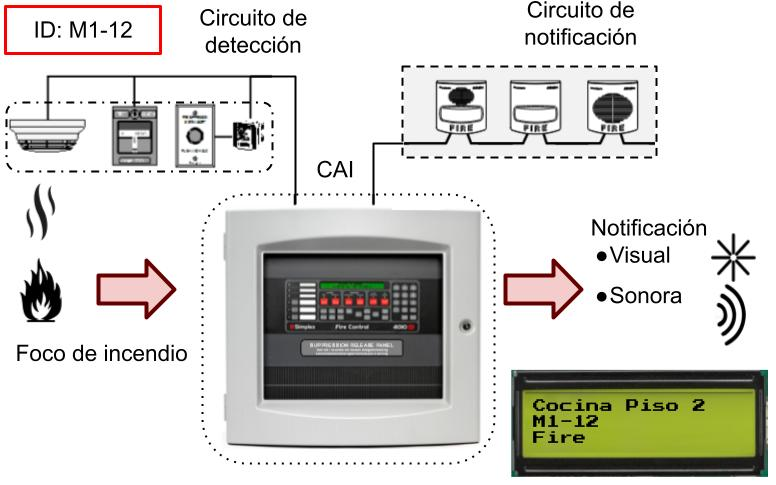
\includegraphics[scale=.45]{./Figures/flujo_conv.jpg}
    \caption{Flujo en caso de un evento de alarma.}
    \label{fig:flujo_conv}
\end{figure}


\subsection{Sistemas de detección de alarma de incendio propuesto}
%
La estructura descrita en la figura \ref{fig:sdai_conv} comprende un SDAI básico, cuenta con lo mínimo requerido para establecer un esquema de protección. Generalmente para instalaciones pequeñas estos servicios suelen ser suficientes, pero existen factores que incrementan las exigencias de protección como por ejemplo: grandes superficies a proteger, múltiples zonas de riesgo en una misma instalación, zonas con diferentes niveles de propagación de incendio, etc. Estos factores hacen necesario que los fabricantes diseñen equipos con la posibilidad de expandir su rango de trabajo e incluso incluir nuevas funcionalidades.

Uno de los factores clave en el diseño de una CAI es la usabilidad, el sistema debe indicar de forma simple y eficiente la aparición de un evento. Esta interfaz debe ser clara con respecto a la información proveniente de un dispositivo de detección, pero también debe permitir al usuario ejecutar comandos de manera rápida según el procedimiento de evacuación. No obstante, los SDAI se rigen por un marco normativo \citep{nfpa_1}, que a pesar de tener diferentes beneficios (como la estandarización de los procesos), a la vez requiere que el usuario conozca la terminología y procedimientos utilizados por la NFPA (National Fire Protection Association) \citep{nfpa_2}. 

Las normas y leyes vigentes exigen capacitaciones regulares con respecto al uso de los SDAI, sin embargo existen algunos factores como: el idioma, error humano, horarios de trabajo, rotación de personal, entre otras.  Que hacen muy improbable que una persona correctamente capacitada se encuentre presente en el la instalación al momento de que ocurra un evento. En la figura \ref{fig:flujo_conv_user} se puede observar el flujo de acciones que debería realizar una persona correctamente capacitada.

\begin{figure}[ht]
    \centering
    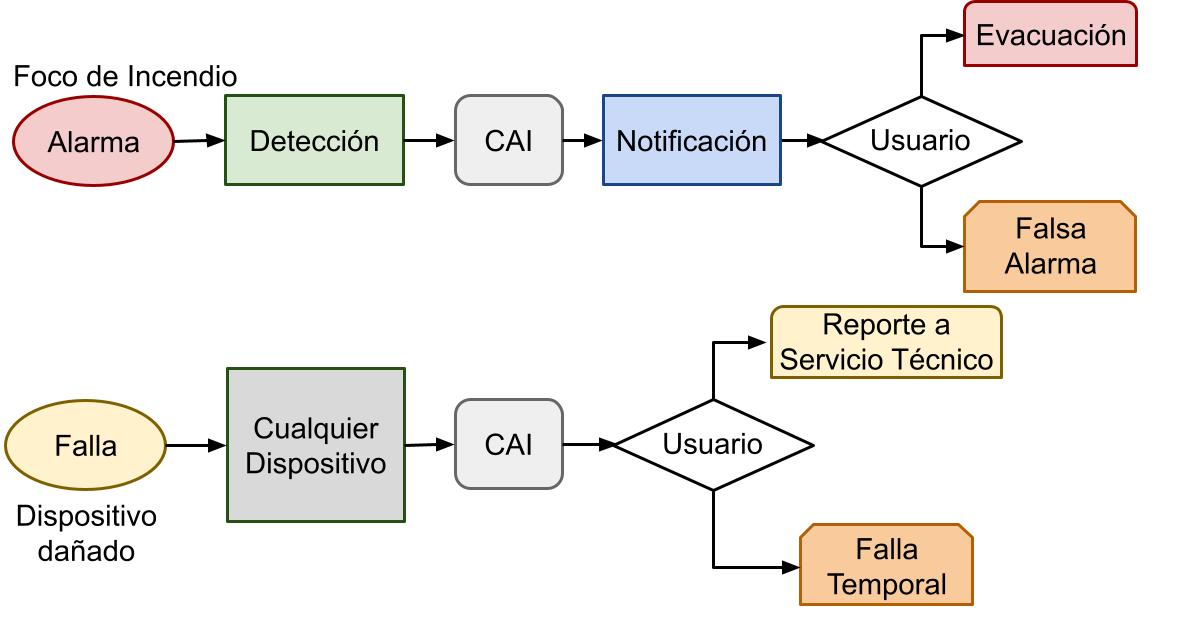
\includegraphics[scale=.3]{./Figures/flujo_dec.jpg}
    \caption{Flujo recomendado para el usuario en caso de eventos.}
    \label{fig:flujo_conv_user}
\end{figure}

Como se puede apreciar en la figura \ref{fig:flujo_conv_user}, el individuo es un elemento indispensable dentro del protocolo de evacuación. El SDAI puede de forma automática detectar y avisar ante focos de incendio, sin embargo las decisiones que se toman en esos primeros minutos afectan directamente el tiempo de reacción, cualquier error, confusión o inclusive inacción por parte del operario puede obstaculizar el éxito de la evacuación \citep{plan_evac}.

La figura \ref{fig:flujo_prop} representa al sistema propuesto, la diferencia radica en que se incluye un módulo de comunicación adicional, que establece conectividad con un servicio alocado en la nube. De esta forma es posible reportar de manera remota cualquier evento presente en el SDAI, no solo a las personas dentro de la instalación que puedan atender a las notificaciones de la central, sino también aquellas personas que interpretan un rol clave al momento de emergencias que puedan no estar al tanto de la situación. Por otro lado, en caso de producirse fallas en cualquiera de los circuitos antes mencionados, la notificación remota puede incluir al personal de mantenimiento. 

\begin{figure}[ht]
    \centering
    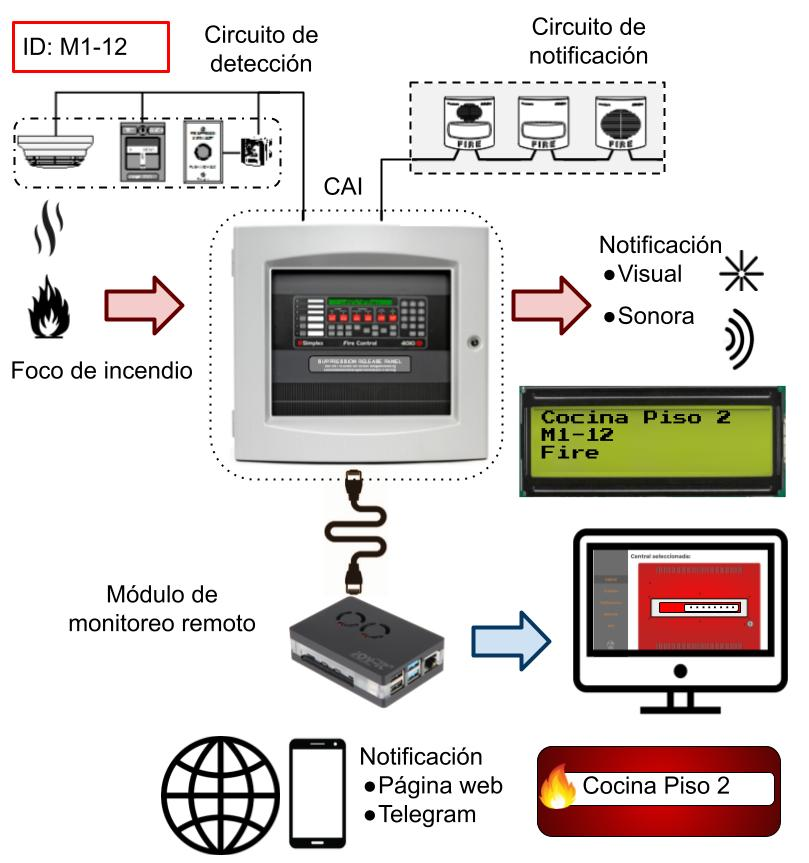
\includegraphics[scale=.45]{./Figures/flujo_prop.jpg}
    \caption{Flujo en caso de un evento de alarma, para el sistema propuesto.}
    \label{fig:flujo_prop}
\end{figure}

\section{Estado del arte}
%

En la tabla \ref{tab:comp} se comparan algunas de las alternativas comerciales. Todas las opciones se enfocan en incrementar el alcance de las notificaciones, sin embargo difieren según la marca del fabricante.

Por lo general cada fabricante cuenta con un protocolo de comunicación que permite a la CAI interactuar con el mundo exterior. Este protocolo suele ser RS232 o en algunos casos Telnet, sin embargo el formato de la información varía entre fabricantes. Es por esto que los sistemas de monitoreo remoto multi-plataforma suelen sacrificar la cantidad de información disponible de los eventos, de lo contrario se verían en la obligación de generar un esquema de decodificación por cada fabricante o incluso en algunos casos por cada modelo (como en el ítem 4 de la tabla \ref{tab:comp}). Desde otro punto de vista, si se incluye menor detalle por cada evento, es posible desarrollar un esquema multiplataforma que recolecte la información y la plasme sin necesidad de segmentarla (similar al ítem 1 de la tabla \ref{tab:comp}).

En un trabajo de investigación previo se desarrolló un sistema de monitoreo de CAI generales, este sistema permite conocer a un nivel básico el estado del SDAI (estado de alarma, falla o normal). El trabajo actual se enfoca en ampliar la cantidad de información que se presenta actualmente en la plataforma de monitoreo, un nivel completo de notificación incluye específicamente los siguientes detalles por dispositivo en caso de presentarse una anomalía o alarma: código, etiqueta, tipo y estado.



\begin{table}[h]
\centering
\caption[caption corto]{Comparación entre equipos comerciales actuales.}
\begin{tabular}{l c c c c c}
\toprule
\textbf{Nombre} & \textbf{Compatibilidad}& \textbf{Nivel de detalle}& \textbf{Ref}\\
\midrule
SNAI (CESE) & Múltiple & Básico & \citep{cese} \\
Safelinc & Simplex & Completo & \citep{safelinc} \\
HT-7001 & Múltiple & Básico & \citep{ht7001}\\
ONYXWORKS & Notifier & Completo & \citep{onyxworks}\\
Control Room Monitor & Múltiple & Completo & \citep{nimbus} \\
Security Server & Bosch & Completo & \citep{ss_bosch} \\
Fire Alarm Monitoring & Múltiple & Básico & \citep{churches}\\
Discador telefónico DT-14 & Múltiple & Básico & \citep{dt_14}\\
\bottomrule
\hline
\end{tabular}
\label{tab:comp}
\end{table}

El sistema comercial que mejor cumple con los objetivos de este trabajo es el sistema de la marca Nimbus \citep{nimbus}. Está orientado al monitoreo multiplataforma, es capaz de indicar con gran nivel de detalle los eventos y cuenta con notificación remota. Las notificaciones remotas se realizan mediante la App de la empresa Nimbus, la cual además cuenta con notificaciones configurables según lo requiera el usuario.

La tabla \ref{tab:comp_cese} compara el proyecto Nimbus con el trabajo actual, ambos sistemas cumplen con un nivel de detalle completo, sin embargo el equipo Nimbus cuenta con un desarrollo más completo al ser multiplataforma e incluir el servicio de identificación de eventos en planos. Sin embargo, la interfaz desarrollada cuenta con bidireccionalidad y la posibilidad de incluir comandos automáticos para un protocolo de pruebas y diagnóstico de la instalación. Además al subir la información a la nube, el sistema tiene el potencial de expandir sus funcionalidades, por lo que herramientas como: diagnóstico preventivo, servicios de notificacion en planos, análisis de fallas y recomendaciones de stock preventivo son posibles. Estas funcionalidades requieren el desarrollo de la interfaz gráfica únicamente ya que no requieren de ningún hardware adicional. 


\begin{table}[h]
\centering
\caption[caption corto]{Comparación entre sistema Nimbus y el trabajo actual.}
\begin{tabular}{l c c c c}
\toprule
\textbf{Nombre} & \textbf{Compatibilidad}&  \textbf{Planos} &\textbf{Bidireccional}\\
\midrule
Trabajo actual & Simplex & Posible & No \\
Control Room Monitor & Múltiple & Sí & No \\
\bottomrule
\hline
\end{tabular}
\label{tab:comp_cese}
\end{table}


\section{Motivación}
%
La firma Isolse srl se dedica a la venta e instalación de sistemas de seguridad electrónica, principalmente en el área de detección y supresión de incendios; cuenta además con una amplia gama de clientes repartidos en a lo largo el territorio nacional, esto hace necesario mantener una movilización constante de su personal técnico.

Este proyecto forma parte del compromiso de desarrollo tecnológico e innovación de la empresa. El propósito de esta investigación es atender una necesidad del mercado argentino: “conocer el estado de los establecimientos protegidos, sin necesidad de trasladarse al sitio”. Es por ello que se desea ampliar los servicios que brinda la empresa, al brindar a sus clientes notificaciones ante cambios en el estado del sistema de detección de incendios de las infraestructuras contratadas. Adicionalmente, conocer el detalle de la instalación previo a una visita de mantenimiento, permite mayor eficiencia en el servicio al cliente, registros históricos de los eventos, análisis de fallas  e incluso propuestas comerciales orientadas en base a los eventos presentes al momento de contactar con el cliente.

Isolse srl recientemente logró ser reconocido como representante oficial de la marca Simplex en Argentina, por lo que los nuevos proyectos e instalaciones se orientan a las prestaciones de la marca. Cada fabricante cuenta con procedimientos de configuración e instalación diferentes, por lo que incluir un nuevo fabricante en el portafolio de trabajo requiere de un programa de capacitaciones. Se debe establecer un procedimiento que permita familiarizar al personal técnico con el conjunto de instrucciones necesarias para la ejecución de tareas de resolución de fallas, simulacros e instalación de nuevos dispositivos. 

\chapter{Introducción específica} % Main chapter title

\label{Chapter2}

%----------------------------------------------------------------------------------------
%    SECTION 1
%----------------------------------------------------------------------------------------
En este capítulo se detallan las tecnologías utilizadas para el desarrollo del firmware, software y las plataformas necesarias para el funcionamiento del sistema.

\section{Centrales de alarma de incendio Simplex}
En los SDAI es común que los fabricantes incluyan un puerto para comunicación con dispositivos externos de registro de eventos, como por ejemplo impresoras. Estos puertos usualmente utilizan el protocolo RS232 \citep{rs232}, lo que hace posible registrar la información en un protocolo estándar en el ámbito industrial y de sistemas embebidos. En el caso de la marca Simplex, adicional a este puerto se incluye una terminal de comandos Telnet \citep{telnet} que obedece a un set de comandos. Esta interfaz sirve como herramienta de depuración durante la instalación de la CAI. Los comandos permiten confirmar elementos de programación tales como el accionamiento de los dispositivos de notificación, la ejecución del protocolo de evacuación, la información de todos los dispositivos instalados, y diversas funcionalidades avanzadas.

El uso de los comandos y su correcta interpretación requiere horas de capacitación y práctica, por lo que se podría considerar que existe una curva de aprendizaje considerable para el manejo de esta terminal. Esto se debe principalmente a que se requiere contar con conocimientos en diferentes aspectos del equipo como: el lenguaje de programación que utiliza, la nomenclatura del fabricante, el set de comandos de la marca, la estructura del programa en texto estructurado y la nomenclatura regulada de la NFPA, entre otros.  El acceso a este puerto suele recomendarse posterior a la segunda capacitación técnica oficial de la marca Simplex debido a su complejidad. En la figura \ref{fig:telnet} se puede observar un esquema que explica el funcionamiento del puerto.

\begin{figure}[ht]
   \centering
   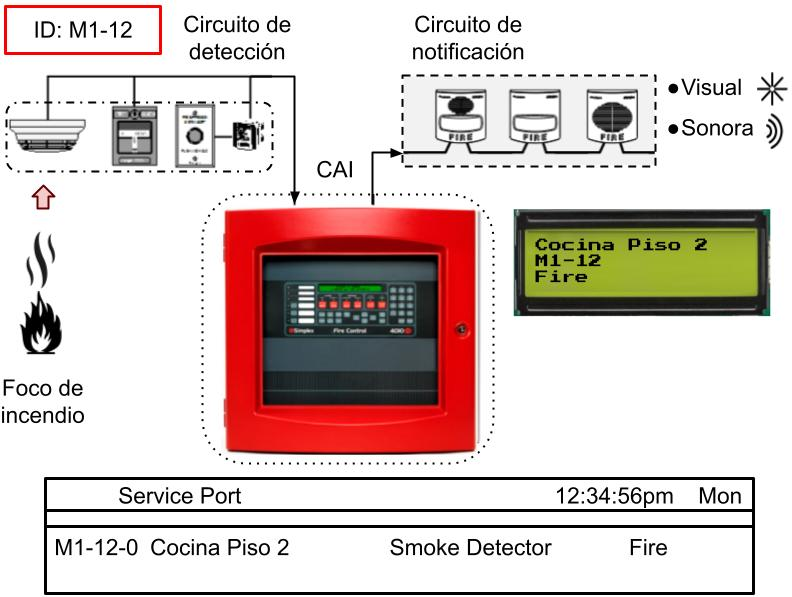
\includegraphics[scale=.45]{./Figures/telnet.jpg}
   \caption{Diagrama de notificaciones mediante puerto de servicio.}
   \label{fig:telnet}
\end{figure}


Considerando las características detalladas, el sistema actual se enfoca en el uso del puerto de comunicación Telnet para expandir los servicios a brindar por el SMAI. Al utilizar el puerto Telnet, se puede disponer de una plataforma que extraiga el detalle de los eventos de la central, y los facilite al usuario mediante Firebase. El objetivo principal es desarrollar un sistema de monitoreo de la CAI con el mayor detalle posible, pero a la vez es de especial interés facilitar el uso de esta plataforma para acelerar las tareas de instalación y mantenimiento de los SDAI Simplex.


\section{Sistema de monitoreo propuesto}

El sistema de monitoreo de alarma de incendio que se propone se compone de diferentes módulos. Como se puede observar en la figura \ref{fig:modulo}, cada módulo hace uso de una herramienta particular con los siguientes objetivos:

\begin{itemize}
\item \textit{Single Board Computer}: plataforma de desarrollo de hardware abierto con soporte para Linux embebido. Las plataformas utilizadas cuentan con soporte de sus comunidades, gran cantidad de tutoriales y documentación. \citep{bbb}.
\item Node-RED: herramienta de programación por bloques que permite la rápida integración de tecnologías y dispositivos. La herramienta permite integrar funcionalidades y servicios de forma sencilla, robusta y escalable. \citep{nodered}.
\item SQLite: biblioteca de funcionalidades que permite generar un motor de búsqueda SQL. El uso de bases de datos permite registrar la información de los eventos y generar un respaldo local de los eventos en caso de fallas de conexión a internet. \citep{sqlite}.
\item Firebase: plataforma enfocada en el desarrollo rápido de aplicaciones y servicios web que brinda un set completo de servicios. Permite incluir nuevas funcionalidades en pocos pasos y asegura la compatibilidad con todos los servicios suministrados por un mismo proveedor. \citep{fbase}.
\item Telegram: aplicación de mensajería que se utiliza como alternativa de notificación remota. Provee una estructura respaldada de mensajería instantánea que permite la notificación rápida al usuario.\citep{telegram}.
\end{itemize}


\begin{figure}[ht]
   \centering
   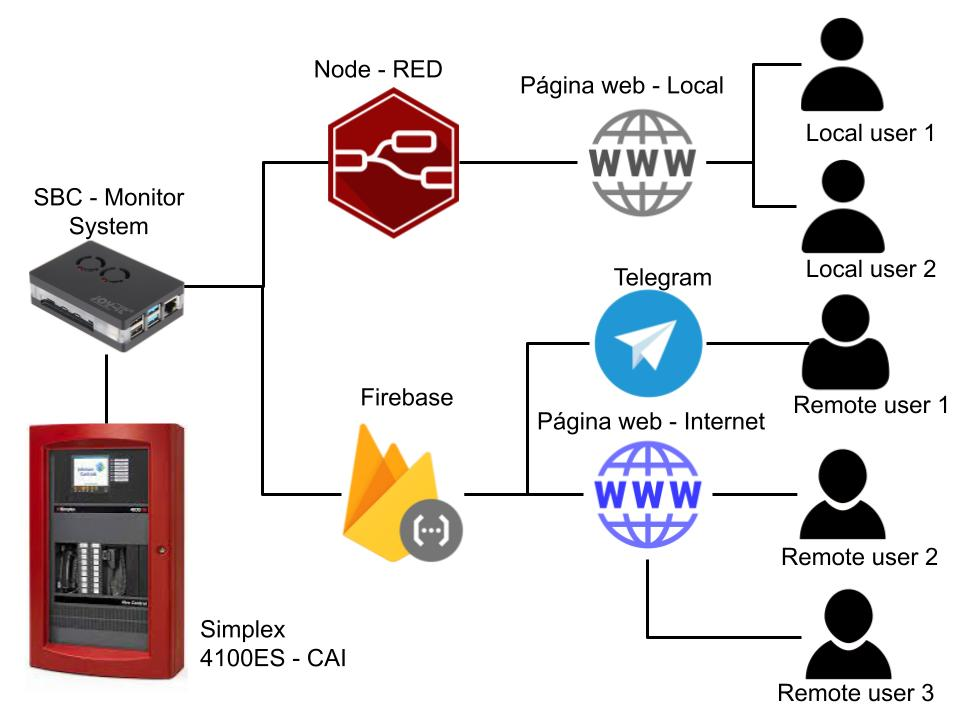
\includegraphics[scale=.35]{./Figures/modulo.jpg}
   \caption{Esquema resumido del sistema de monitoreo.}
   \label{fig:modulo}
\end{figure}


\section{Plataformas de desarrollo utilizadas}

\subsection{Plataforma de desarrollo web: Firebase}
Firebase es una plataforma alojada en la nube, que facilita el desarrollo de aplicaciones web y además integra diferentes servicios como:
\begin{itemize}
\item Autenticación: solución al control de acceso de usuarios, set de herramientas que gestionan el acceso de los usuarios de forma segura e incluso la recuperación de credenciales.
\item Base de datos en tiempo real: sistema de gestión de datos que facilita la sincronización de la información en todos los dispositivos con el acceso correspondiente.
\item Almacenamiento: servicio de almacenamiento de todo tipo de archivos. De gran utilidad para el intercambio de archivos como manuales, diagramas e ilustraciones por aprte del bot.
\item \textit{Hosting}: servicio que implementa y mantiene disponible las páginas web requeridas para el reporte de información mediante la web.
\item Funciones: servicio de ejecución de programas y automatizaciones configurables. Se utiliza para realizar el procesamiento de la información y la coordinación del reporte de eventos al resto de servicios.
\end{itemize}

La figura \ref{fig:d_fbase} muestra un esquema de los servicios de Firebase utilizados en el proyecto y su contribución. Los servicios más importantes a resaltar son el de funciones y la base de datos en tiempo real. Entre ambos servicios permiten incluir al sistema diferentes funcionalidades y coordinan los reportes de notificacion.

\begin{figure}[ht]
   \centering
   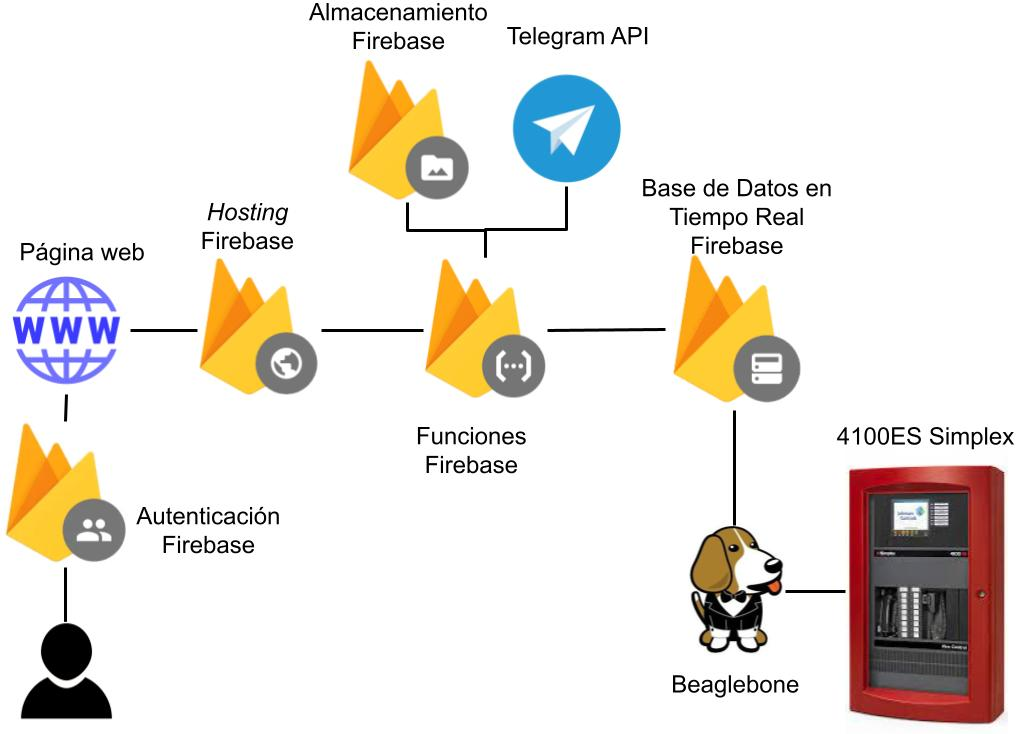
\includegraphics[scale=.35]{./Figures/d_fbase.jpg}
   \caption{Esquema de servicios de Firebase.}
   \label{fig:d_fbase}
\end{figure}



\subsection{Hardware de desarrollo}

En primera instancia, el sistema se continua en una Raspberry Pi 3 B + para el desarrollo de los programas, la interfaz de usuario, la validación de la estructura y el flujo de trabajo. Sin embargo, debido al feedback de expertos al finalizar el trabajo de investigación \citep{cese}.

Basados en la experiencia durante el cursado de la maestría se decide implementar el sistema en una placa Beaglebone Black \citep{bbb}, con el objetivo de incrementar la robustez del sistema y enfocar el desarrollo a un producto final. Adicional a las mejoras de hardware, también tenemos la posibilidad de compilar de forma cruzada nuestra propia versión de Linux con las características requeridas para el sistema.

\subsection{Herramienta de desarrollo de interfaz gráfica: Node-RED}

Herramienta de programación en bloque compatible con diferentes sistemas de bajo recursos. Simplifica la integración de dispositivos de hardware a través de módulos listos, que implementan los protocolos de comunicación más comunes en el ámbito industrial y de desarrollo. Además incluye módulos de generación de interfaces de usuario, que en pocos minutos establecen un servicio de hosting local con el objetivo de proveer un método de visualización y comando a partir de dispositivos con navegadores web. 

\subsection{Servicio de mensajería instantánea: Telegram}

Telegram corresponde al servicio de mensajería seleccionado para notificar a los usuarios de la presencia de un evento en su recinto. Telegram permite desarrollar de forma gratuita bots basados en su API, lo que brinda una atención más personalizada a los usuario y, adicionalmente, permite segmentar los servicios que proveen de forma clara. Si en dado caso se requiriera implementar nuevas funcionalidades, el esquema de trabajo de bots permite incorporar nuevas funcionalidades de forma sencilla, con la opción de habilitarlas sólo cuando estén funcionales y hayan sido testeadas correctamente.
 
\include{Chapters/Chapter3}
\include{Chapters/Chapter4} 
% Chapter Template

\chapter{Conclusiones} % Main chapter title

\label{Chapter5} % Change X to a consecutive number; for referencing this chapter elsewhere, use \ref{ChapterX}

En esta sección se detalla el nivel de cumplimiento de los requerimientos como así también los principales aportes del trabajo realizado. Se describen adicionalmente aspectos en los que el sistema puede evolucionar.

%----------------------------------------------------------------------------------------

%----------------------------------------------------------------------------------------
%	SECTION 1
%----------------------------------------------------------------------------------------

\section{Resultados obtenidos}


Basados en la primera versión del sistema de monitoreo de centrales de alarma de incendio (SMCAI) desarrollado como trabajo final de la CESE, se logró implementar de forma exitosa un sistema de monitoreo remoto, que describe en detalle el estado de una central de alarma de incendio de la marca Simplex (SMCAI-S).

El nivel de detalle que proporciona el SMCAI-S, es debido a que utiliza la interfaz de comandos Telnet de la marca Simplex. De esta manera se establece una interfaz que provee las siguientes funcionalidades:
\begin{itemize}
\item Monitoreo detallado del estado del sistema de detección de incendios.
\item Interfaz web con acceso desde cualquier parte del mundo.
\item Servicio de mensajería instantánea a través de un bot de Telegram.
\item Plataforma funcional y escalable sin restricciones asociadas al número de centrales.
\end{itemize}

Actualmente el SMCAI-S se ejecuta en un hardware orientado a prototipado y uso general, lo que brindó la flexibilidad necesaria para disminuir los tiempos de desarrollo. Elemento clave para definir un producto mínimo viable junto con los colaboradores de la empresa Isolse srl. Sin embargo, se considera que para efectos comerciales, es recomendable contar con un sistema de hardware propio basado en los requerimientos.

A partir del análisis de la normativa de incendio NFPA 72, se diseñó un esquema de conectividad que resguarda la integridad de la CAI. Asimismo, el esquema considera que además de la interconectividad, un punto crítico del sistema es la conexión a la red, es por ello que el análisis de riesgos del sistema impulsó la incorporación de una conexión redundante a la red. 

La combinación de este trabajo (SMCAI-S) en conjunto con el sistema realizado previamente (SMCAI), proporcionan una plataforma de monitoreo sumamente completa con las siguientes características:
\begin{itemize}
\item CAI de marca diferente a Simplex: se indica la condición de la central mediante los estados de alarma, falla o normal.  
\item CAI de marca Simplex: se brinda un detalle completo de todos los eventos que se presenten, a través de la siguiente nomenclatura por cada dispositivo:
\begin{itemize}
	\item ID: corresponde a un código único por dispositivo.
	\item Etiqueta: texto de 40 caracteres nomenclados en base a la ubicación física del dispositivo en la instalación.
	\item Tipo: tecnología de detección utilizada por el dispositivo.
	\item Estado: texto descriptivo de la condición presente en el dispositivo.
\end{itemize}
\end{itemize}

Finalmente, debido a complicaciones con la importación de equipos y la apremiante necesidad de una alternativa de monitoreo, el foco del trabajo fue el monitoreo remoto. Por consecuencia objetivos asociados a funcionalidades de mantenimiento y soporte durante el proceso de instalación fueron desestimados por el momento. 



%----------------------------------------------------------------------------------------
%	SECTION 2
%----------------------------------------------------------------------------------------
\section{Trabajo futuro}

Los trabajos de investigación tecnológica de la empresa Isolse SRL tienen como objetivo innovar dentro del mercado de detección de incendios. En estos momentos los trabajos se orientan al diseño de sistemas y plataformas de validación, es decir prototipos que permitan validar los planteamientos creativos con la finalidad de concretar una propuesta comercial.

A continuación se listan los próximos pasos a seguir para lograr una propuesta comercial sólida con el sistema actual:
\begin{itemize}
\item Diseño de hardware específico, con foco en la certificación del producto.
\item Mejoras al esquema de servicio multi-cliente para el bot de Telegram.
\item Incorporación de documentación y guías de ayuda adicionales para el menú de ayuda del bot en Telegram.
\item Implementación de tareas de mantenimiento, prueba y validación de la instalación de las CAI de marca Simplex.
\item Incluir la decodificación de los protocolos de comunicación de otras marcas comerciales de CAI.
\end{itemize}

Una vez obtenida una propuesta comercial viable, se abre una nueva línea de investigación y desarrollo tecnológico. El objetivo de esta investigación es aprovechar la información registrada por la plataforma actual, y brindar nuevos servicios como:
\begin{itemize}
\item Sistema de análisis de fallas predictivo.
\item Sistema de mantenimiento preventivo.
\item Herramienta de análisis de calidad de instalación.
\item Sistema de monitoreo basado en los planos de la instalación.
\item Integración de servicios de monitoreo de terceros.
\item Aplicación para dispositivos móviles.
\item Integración con softwares comerciales de gestión de edificios, por ejemplo marcas como: Siemens, Honeywell, Johnson Controls.
\end{itemize}
 

%----------------------------------------------------------------------------------------
%	CONTENIDO DE LA MEMORIA  - APÉNDICES
%----------------------------------------------------------------------------------------

\appendix % indicativo para indicarle a LaTeX los siguientes "capítulos" son apéndices

% Incluir los apéndices de la memoria como archivos separadas desde la carpeta Appendices
% Descomentar las líneas a medida que se escriben los apéndices

%\include{Appendices/AppendixA}
%\include{Appendices/AppendixB}
%\include{Appendices/AppendixC}

%----------------------------------------------------------------------------------------
%	BIBLIOGRAPHY
%----------------------------------------------------------------------------------------

\Urlmuskip=0mu plus 1mu\relax
\raggedright
\printbibliography[heading=bibintoc]

%----------------------------------------------------------------------------------------

\end{document}  
